\documentclass[12pt]{article}
\usepackage[a4paper, margin=.30in]{geometry}
%\usepackage{array}
\usepackage{fancybox}
\usepackage{pgfplots}
\pgfplotsset{compat=1.18} % Version de PGFPlots
\usepackage{tikz}
\usepackage{filecontents}
\usepackage{graphicx, subfig, wrapfig, makecell,multirow }
\newcommand\headerMe[2]{\noindent{}#1\hfill#2}
\renewcommand \thesection{\Roman{section}}

\newcolumntype{M}[1]{>{\raggedright}m{#1}}




\begin{document}

\headerMe{Royaume du Maroc}{année scolaire \emph{2024-2025}}\\
\headerMe{Ministère de l'Éducation nationale, }{  Professeur :\emph{Zakaria Haouzan}}\\
\headerMe{du Préscolaire et des Sports}{Établissement : \emph{Lycée SKHOR qualifiant}}\\

\begin{center}
Devoir surveillé N°2-S1 \\
Durée 2h00\\
\underline{2-BAC Section des sciences Mathématiques}\\

    \vspace{.2cm}
\hrulefill
\Large{Fiche Pédagogique}
\hrulefill\\
\end{center}
%end Headerss------------------------


%__________________Chimie ______________________-
%%%%%%%+_+_+_+_+_+_+_+_+_Partie1
\section[A]{Introduction }
\hspace{0.5cm}Le programme d'études de la matière physique chimie vise à croître un ensemble de compétences visant à développer la personnalité de l'apprenant. Ces compétences peuvent être classées en Compétences transversales communes et Compétences qualitatives associées aux différentes parties du programme.
\section{cadre de référence }
 \hspace{0.5cm}L'épreuve a été réalisée en adoptant des modes proches à des situations d'apprentissages et des situations problèmes, qui permettent de compléter les connaissances et les compétences contenues dans les instructions pédagogiques et dans le programme de la matière physique chimie et aussi dans le cadre de référence de l'examen national. 
 \\Tout en respectant les rapports d'importance précisés dans les tableaux suivants :
 \begin{center}
\begin{tabular}{|c||c||c|}
\hline
    \textbf{Restitution des Connaissances} & \textbf{Application des Connaissances} & \textbf{Situation Problème }\\
    \hline 
    $40\%$ & $30\%$ & $30\%$\\
    \hline
\end{tabular} 
\end{center}

\section{tableau de spécification}
 \begin{center}
\begin{tabular}{||c|c||c|c|c|c|}
\hline
     \multicolumn{2}{||c||}{\bf{   \hfill  Niveau d'habileté  \hfill } }
	& \makecell{Restitution \\des Connaissances} &\makecell{Application \\des Connaissances} & \makecell{Situation Problème} & la somme \\\hline

	%  
	\multirow{1}{*}{\makecell{Transformations \\nucléaires 62\%}}
	& \makecell{Décroissance\\radioactive\\17\%}  & \makecell{7\%\\4Q - 4pts}  &\makecell{5\%\\2Q - 2pt} & \makecell{5\%\\1Q - 1pt} & 

	\multirow{3}{*}{\makecell{62\%\\13pts\\12Q\\75min}}\\\cline{2-5}
  & \makecell{Noyaux,\\masse\\et énergie \\45\%}  & \makecell{18\%\\2Q - 2pts}  &\makecell{15\%\\2Q - 2pt } & \makecell{14\%\\1Q - 1pt} &\\\hline

%& \makecell{Les Ondes \\lumineuse}  & \makecell{10\%\\3Q - 3pts}  &\makecell{5\%\\1Q - 1pt } & \makecell{5\%\\2Q - 1pt} &\\\hline

\multirow{2}{*}{ \makecell{Les\\Transformations\\non totales d'un\\d'un\\système\\chimique 47\%}}

& \makecell{Transfo\\chimiques\\dans les\\deux sens}  & \makecell{\\18\%\\6Q - 4pts}  &\makecell{14\% \\2pts - 2Q } & \makecell{13\%\\2pts - 2Q} &

\multirow{1}{*}{\makecell{38\%\\7pts\\10Q\\45min }}\\

& \makecell{État\\d’équilibre\\d’un\\système\\chimique}  & \makecell{}  &\makecell{} & \makecell{} &\\\hline



     \multicolumn{2}{||c||}{\bf{   \hfill  --  \hfill } }
& \makecell{40\%\\14Q - 11pts}  &\makecell{30\%\\6Q - 5pts } & \makecell{30\%\\6Q - 5pts} &\\\hline



\end{tabular} 
\end{center}

\newpage
\begin{center}
    \shadowbox{\bf{ Devoir surveillé $N^{\circ}$1 Semestre I} }
\end{center}
 \begin{center}

     \begin{tabular}{|c||c||c|}
    \hline
         \multicolumn{3}{||c||}{\bf{   \hfill  Chimie  \hfill (7pts)} }\\
         \hline
         \multicolumn{3}{||c||}{\bf{Suivi temporel d’une transformation chimique par la conductimétrie\dotfill} }\\
\hline
    \textbf{$N^{\circ}$Question } & \textbf{Réponse } & \textbf{Note }\\
    \hline
    $1.$ &
         \makecell{les quantités de matière initiales des réactifs.\\
			 $n_0(Zn_{(s)}) = 0,016 mol$ et $n_0(H_3O^+_{(aq)}) = 0,04mol$
 }
    & $0,5pts$\\\hline
 %Q2
     $2.$ &
     \makecell{
		 le tableau d’avancement de cette réaction.\\
 \begin{tabular}{|c|c|c|c|c|c|}
    \hline
	\multicolumn{2}{|c|}{Equation de la réaction}& \multicolumn{4}{c|}{$2H_3O^+$ + Zn $\rightarrow$ $Zn^{2+}$ + $2H_2O$}\\\hline
    états  & avancement& \multicolumn{4}{|c|}{quantité de Matière en mol}\\\hline
    Etat initial          &    0        &  0,04&0,01&  0              &  0 \\\hline
\makecell{Etat de \\transformation}&$x$ & $0,04-2x$ & $ 0,01-x$ & $x$  & $x$ \\\hline
    Etat final&    $x_{max}$& $ 0,04 - 2x_{max}$ & $0,01 - x_{max}$ & $2x_{max}$  & $x_{max}$ \\\hline
   % \cline{2-4}\
\end{tabular}\\
	 }
    & $0,5pts$\\\hline  
 %Q3
     $3$ &
	 \makecell{ $x_{max} = 0,016mol$ et le réactif limitant Zn.}
    & $0,5pts$\\\hline  
 %Q4
     $4$ &
         \makecell{la diminution de la conductivité mesurée au cours de la transformation chimique
\\est due à la disparition des ions $H_3O^+$ }
    & $0.25pt$\\\hline  
 %Q5
     $5$ &
	 \makecell{$\sigma = 21,3 - 7,42.10^2x$ }
    & $1pt$\\\hline  
      
	 $6$ &
	  \makecell{a t = 400s x = 0,014mol donc $n(H_3O^+)_t=0,012mol$ ; $n(Zn)_t=0,002mol$ ;\\ $n(Zn^{2+})_t = n(H_2)_t = 0,014mol$ et $V(H_2)=3,5L$  }
    & $1,25pts$\\\hline  

    $7$ &
	\makecell{’expression de v la vitesse volumique $v =-\frac{1}{7,42.10^2.V}.\frac{d\sigma}{dt} $ \\et $v(t=0) =0,842 S/m^4 $; $v(t=400)=0,168 S/m^4 $ }
    & $1pt$\\\hline  
 %Q5
     $8$ &
	 \makecell{a t=$t_{1/2}$ $\sigma_t{1/2} = 15S/m$  donc $t_{1/2} = 160s$ }
    & $0,25pt$\\\hline  
  %Q5
     $9$ &
	 \makecell{ l'évolue la vitesse de réaction au cours du temps et Donner \\une interprétation de cette variation en envisageant un facteur cinétique.}
    & $0,25pt$\\\hline  
 
 %Q5
     $10$ &
	 \makecell{Tracer , en justifiant , sur le même courbe précédente , l’allure de \\la courbe obtenue dans ce cas. }
    & $1,5pt$\\\hline  
 
%%Partie 2 : 
         %\multicolumn{3}{||c||}{\bf{Partie 2 : Suivi d’une transformation chimique\dotfill (2pts)}}\\
%\hline
%$1.$ &
         %\makecell{\\ % table dont forget 
             %\begin{tabular}{|c|c|c|c|c|c|}
    %\hline
    %\multicolumn{2}{|c|}{Equation de la réaction}& \multicolumn{4}{c|}{2CuO + C $\rightarrow$ 2Cu + $CO_2$}\\\hline
    %états  & avancement& \multicolumn{4}{|c|}{quantité de Matière en mol}\\\hline
    %Etat initial          &    0        &  12.38 &  1.4&  0              &  0 \\\hline
                 %\makecell{Etat de \\transformation}&    $x$      & $ 12.38 - 2x$ & $ 1.4 - x$ & $ 2x$  & $x$ \\\hline
    %Etat final            &    $x_{max}$& $ 12.38 - 2x_{max}$ & $1.4 - x_{max}$ & $2x_{max}$  & $x_{max}$ \\\hline
   %% \cline{2-4}\
%\end{tabular}
         %\\$\; $ }  
    %& $1pt$\\\hline
 %%Q2
   %$2$ &
         %\makecell{ l’avancement maximal $x_{max} = 1.4mol$ et le réactif limitant le carbone C(s) 
 %}
    %& $0.5pt$\\\hline  
 %%Q3
   %$3$ &
         %\makecell{ bilan de matière dans l’état final :\\ $n_f(CuO) = 9.58 mol$ et $n_f(C) = 0 mol$ et $n_f(Cu) = 2.8 mol$, $n_f(CO_2) = 1.4mol$ 
 %}
    %& $0.5pt$\\\hline  
%Physique : 
    %Partie 1 : 
\end{tabular} 
\end{center}

\begin{center}
  \begin{tabular}{|c||c||c|}
    \hline
         \multicolumn{3}{||c||}{\bf{   \hfill  Physique  \hfill (13pts)} }\\
         \hline
         \multicolumn{3}{||c||}{\bf{Partie 1 : le mouvement des vagues \dotfill (3pts)} }\\
\hline
    \textbf{$N^{\circ}$Question } & \textbf{Réponse } & \textbf{Note }\\
    \hline
    $1$ &
         \makecell{
			 L’onde étudiée est transversale}
    & $1pt$\\\hline
 %Q2
 $2$ &
         \makecell{ la vitesse de propagation de ces ondes v =10m/s }
    & $1pt$\\\hline
 %Q3
 $3$ &
         \makecell{
			 le nom du phénomène observé diffraction . puis $\lambda = d = 70m$
      }
    & $1pt$\\\hline
      %Partie 2 : -----
\multicolumn{3}{||c||}{\bf{Partie 2 : Propagation d’une onde ultrasonore dans l’air \dotfill (5pts)} }\\
\hline
%1
 $1$ &
 \makecell{ Définir une onde mécanique progressive. }
    & $1pt$\\\hline
%2
 $2$ &
      \makecell{ L’onde ultrasonore est longitudinale }
    & $1pt$\\\hline
%2
 $3$ &
      \makecell{la relation entre la longueur d’onde $v = \lambda.N$ }
    & $1pt$\\\hline
%2
 $4.1$ &
      \makecell{ graphiquement la valeur de la période $T=10.\mu.S$ }
    & $1pt$\\\hline
 $4.2$ &
      \makecell{ la valeur de $\lambda = 3,4cm$ }
    & $1pt$\\\hline

\multicolumn{3}{||c||}{\bf{Partie 2 : Étude du phénomène ondulatoire.\dotfill (5pts)} }\\
\hline
%1
 $1$ &
 \makecell{Nom du phénomène observé diffraction la nature de
la lumière monochromatique }
    & $1pt$\\\hline
%2
 $2$ &
 \makecell{a l’aide de la figure 1 $\theta = \frac{L}{2.D}$ }
    & $0,5pt$\\\hline
 $3$ &
 \makecell{En utilisant les résultats des mesures $\theta = 3,15.10^{-3} rad$ }
    & $0,5pt$\\\hline

 $4$ &
 \makecell{la relation qui lie les grandeurs  $\theta = \frac{\lambda}{a}$ 
}
 
    & $0,5pt$\\\hline
 $5$ &
 \makecell{la valeur de la longueur d'onde  $\lambda = 0,63m$ \\elle appartient au domaine visible 
}
 & $0,5pt$\\\hline

 $6$ &
 \makecell{-on remplace la lumière émise par le LASER (lumière rouge) par une lumière bleue\\L diminue\\
	 -n diminue la largeur de la fente a L augmente\\
	 -différencier expérimentalement une lumière monochromatique d’une lumière \\ polychromatique  par un prisme
}
 & $2pt$\\\hline











  \end{tabular}
  \end{center}



\begin{figure}[h]
    \centering
    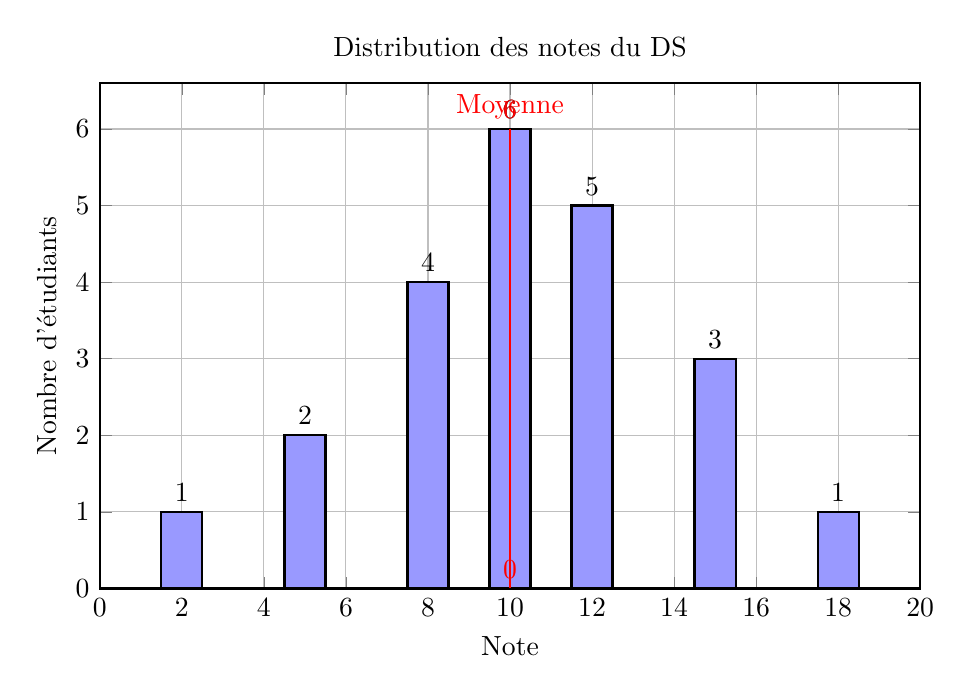
\begin{tikzpicture}
        \begin{axis}[
            width=12cm,
            height=8cm,
            xlabel={Note},
            ylabel={Nombre d'étudiants},
            title={Distribution des notes du DS},
            ymin=0,
            xmin=0,
            xmax=20,
            grid=major,
            % Personnalisation de l'apparence
            thick,
            bar width=1,
            nodes near coords, % Affiche les valeurs au-dessus des barres
        ]
        
        % Données fictives - à remplacer par vos données réelles
        \addplot[ybar, fill=blue!40] coordinates {
            (2,1)  % 1 étudiant avec 2/20
            (5,2)  % 2 étudiants avec 5/20
            (8,4)  % 4 étudiants avec 8/20
            (10,6) % 6 étudiants avec 10/20
            (12,5) % 5 étudiants avec 12/20
            (15,3) % 3 étudiants avec 15/20
            (18,1) % 1 étudiant avec 18/20
        };
        
        % Ligne de la moyenne
        \addplot[red,thick] coordinates {
            (10,0) (10,6)
        } node[above] {Moyenne};
        
        \end{axis}
    \end{tikzpicture}
    \caption{Distribution des notes du DS}
\end{figure}

% Ajout du bilan statistique
\begin{center}
    \begin{tabular}{|l|c|}
        \hline
        \textbf{Statistique} & \textbf{Valeur} \\
        \hline
        Nombre d'étudiants & 22 \\
        Note minimale & 2/20 \\
        Note maximale & 18/20 \\
        Moyenne & 10/20 \\
        Médiane & 10/20 \\
        \hline
    \end{tabular}
\end{center}



\end{document}
